\documentclass{article}

% include graph
\usepackage{graphicx}
% if then else
\usepackage{ifthen}
% for sub itermize
\usepackage{outlines}
% using color package
\usepackage[usenames,dvipsnames]{color}
% 用于产生一种数学用的花体字  
\usepackage{mathrsfs}
% 数学符号  
\usepackage{amsmath,amssymb}
% 专门处理数学粗体的bm宏包
\usepackage{bm}
% 高质量数学字体/黑体  
\usepackage[cmintegrals]{newtxmath}
% Expectation by \E
% just use "\mathbb{E}"
% \DeclareMathOperator{\E}{\mathbb{E}}
% 英文花体, e.g., $\mathcal{D}$
% use table
\usepackage{tabularx}
\usepackage{booktabs}
% use tab
\usepackage{tabto}
% 可以换行的 \underline{}
% \usepackage{ulem} bug: 与emph冲突
% 文字的删除线 \st
\usepackage{soul}
% tickz 画图
\usepackage{tikz}
\usetikzlibrary{graphs}
% for sub figure
\usepackage{subcaption}
% how to write max over x: \max\limits_x

%----------------------------- THE ARTICLE -------------------------------

\begin{document}

\begin{titlepage}
    \includegraphics[height=3.4cm]{../others/sedes.pdf}
    \\ \\
    \textbf{Fundamentals of Artificial Intelligence [H02C1a]}
    \\ \\ 
    \textbf{Xinhai Zou (r0727971)}
\end{titlepage}

\pagenumbering{roman} 
\tableofcontents
\clearpage
\pagenumbering{arabic}
\setcounter{page}{1}

\section{Intro to AI}
\input{01_intro_AI}
\section{Rational agent}
\input{02_rational_agent}
\section{State space}
\input{03_state_space}
\section{Uniformed search}
\subsection{Overview}
Some terminologies for searching problem in graph:
\begin{enumerate}
    \item node expansion: generating all successor node considering the availble actions (the whole process)
    \item explored nodes: nodes that have already been expanded
    \item frontier/ fringe: set of all nodes available for expansion (candidate for expansion)
    \item search stratege: defines which node is expanded next (the strategies)
\end{enumerate}

\noindent
\subsection{Graph search}
Graph search, frontier = {<s,a>, <s,b>}, its \textcolor{blue}{basic} algorithm: \\
\textbf{Input:} \\
\tabto{5mm} a graph, \\
\tabto{5mm} a set of start nodes, \\
\tabto{5mm} Boolean procedure \emph{goal(n)} that tests if \emph{n} is a goal node. \\
\emph{frontier} := {$<s>$, $s$ is a start node} \\
\textbf{while} \emph{frontier} is not empty: \\
\tabto{5mm} \textbf{select} and \textbf{remove} path $<n_{0},...,n_{k}>$ from \emph{frontier} \textbf{for every} neighbor $n$ of $n_{k}$ \\
\tabto{10mm} \textcolor{blue}{\textbf{if} \emph{goal(n)}} \\
\tabto{15mm} \textcolor{blue}{\textbf{return} $<n_{0},...,n_{k},n>$} \\
\tabto{10mm} \textbf{else add} $<n_{0},...,n_{k},n>$ to \emph{frontier} \\
\textbf{end while} \\

\noindent
For loop detection, the \textcolor{red}{loop-detection} algorithm will be: \\
\textbf{Input:} \\
\tabto{5mm} a graph, \\
\tabto{5mm} a set of start nodes, \\
\tabto{5mm} Boolean procedure \emph{goal(n)} that tests if \emph{n} is a goal node. \\
\emph{frontier} := {$<s>$, $s$ is a start node} \\
\textbf{while} \emph{frontier} is not empty: \\
\tabto{5mm} \textbf{select} and \textbf{remove} path $<n_{0},...,n_{k}>$ from \emph{frontier} \textbf{for every} neighbor $n$ of $n_{k}$ \\
\tabto{10mm} \textcolor{blue}{\textbf{if} \emph{goal(n)}} \\
\tabto{15mm} \textcolor{blue}{\textbf{return} $<n_{0},...,n_{k},n>$} \\
\tabto{10mm} \textcolor{red}{\textbf{else if} $n \notin {n_{0},...,n_{k}}$} \\
\tabto{15mm} \textbf{then add} $<n_{0},...,n_{k},n>$ to \emph{frontier} \\
\textbf{end while} \\

Two basic searching strategies for selecting nodes to explore: depth-first search and breadth-first search.

\subsection{DFS and BFS}
\subsubsection{Depth-First Search (DFS)}
Its selecting strategy is \textbf{LIFO = "Last In First Out"}, we work with \textbf{stack}. 
\begin{outline}
    \1 Time complexity: $O(b^{m})$
        \2 with b: branching factor, m: maximum depth
    \1 Space complexity: $O(b \times m)$
        \2 with b: branching factor, m: maximum depth
\end{outline}

\noindent
The property of DFS:
\begin{outline}
    \1 Time complexity: $O(b^{m})$
    \1 Space complexity: $O(b \times m)$
    \1 Completeness: is complete if finite m and prevent loop
    \1 Optimal: no guarantee, it finds the leftmost solution
\end{outline}

\subsubsection{Breadth-First Search (BFS)}
Its selecting strategy is \textbf{FIFO = "First In First Out"}, we work with \textbf{queue}.
\begin{outline}
    \1 Time complexity: $O(b^{s})$
        \2 with b: branching factor, s: shallowest-solution depth
    \1 Space complexity: $O(b^{s})$
        \2 with b: branching factor, s: shallowest-solution depth
    \1 Completeness: no matter loop or not, it is complete
    \1 Optimal: optimal only if \textbf{cost between each node = 1}
\end{outline}

\subsubsection{Comparison of DFS \& BFS}
DFS uses less memory, but needs loop detection; while BFS use more memory, but does not need loop detection. More details are shown as below: \\
\begin{outline}
    \1 Depth-First Search
        \2 Space is restricted
        \2 Many solutions exist, solutions are long
        \2 no infinite paths
    \1 Breadth-First Search
        \2 Space is not a problem
        \2 Solution containing fewest/shallowest depth
\end{outline}

\subsection{Iterative Deepening}
Iterative Deepening is a combinatino of DFS and BFS, the idea is to get advantages from both DFS (space complexity) and BFS (time complexity, optimal, completeness). Run a DFS with depth limit 0/1/2/3/.... (P.S.:LIFO-stack, FIFO-queue). \\
Furthermore, the \textbf{outter} algorithm: \\
\textbf{procedure iterative-deepening (} \\
\tabto{5mm} \textbf{Input:}  \\
\tabto{5mm} a graph, \\
\tabto{5mm} a set of start nodes, \\
\tabto{5mm} Boolean function \emph{goal(n)} that tests if \emph{n} is a goal mode \\
\textbf{)} \\
\emph{depthlimit = 1} \\
\textbf{while} goal not found \textbf{do} \\
\tabto{5mm} call depth-limited-search(graph, starting nodes, \emph{goal(n)}, \emph{depthlimit})
\tabto{5mm} \emph{depthlimit = depthlimit + 1} \\

\noindent
The \textbf{inner} algorithm: \\
\textbf{procedure depth-limited-search(} \\
\tabto{5mm} \textbf{Input:}  \\
\tabto{5mm} a graph, \\
\tabto{5mm} a set of start nodes, \\
\tabto{5mm} Boolean procedure \emph{goal(n)} that tests if \emph{n} is a goal node, \\
\tabto{5mm} \textcolor{red}{\emph{depthlimit}: natural number} \\
\textbf{)} \\
\emph{frontier} := {$<s>$ : $s$ is a start node} \\
\textbf{while} \emph{frontier} is not empty: \\
\tabto{5mm} \textbf{select} and \textbf{remove} \textcolor{red}{first} path $<n_{0},...,n_{k}>$ from \emph{frontier} \\
\tabto{5mm} \textcolor{red}{\textbf{if} \emph{k < depthlimit}} \\
\tabto{10mm} \textbf{for every} neighbor $n$ for $n_{k}$ \\
\tabto{15mm} \textcolor{blue}{\textbf{if} \emph{goal(n)}} \\
\tabto{20mm} \textcolor{blue}{\textbf{then return $n_{0},...,n_{k},n$}} \\
\tabto{15mm} \textbf{else add} $n_{0},...,n_{k},n$ to \textcolor{red}{start of} \emph{frontier} \\
\textbf{end while} \\

\noindent
The property of iterative deepening (ID) is similar to BFS, the only difference is the memory usage which is better than BFS ($O(b \times s) \ge O(b^{s})$). \emph{Time complexity almost is the same as BFS, the only difference is ID needs iterative reconstruction each limit of 0,1,2,3 needs to start from start node (root) and to rebuild the search tree}
\begin{outline}
    \1 Time complexity: $O(b^{s})$
        \2 with b: branching factor, s: shallowest-solution depth
    \1 Space complexity: $O(b \times s)$
        \2 with b: branching factor, s: shallowest-solution depth
    \1 Completeness: no matter loop or not, it is complete
    \1 Optimal: optimal only if \textbf{cost between each node = 1}
\end{outline}

\subsection{Bi-directional search}
Forward and backward search together. But it is not always possible \emph{because backward is not always known}. The algorithm is shown below: \\
\textbf{Input:} \\
\tabto{5mm} a graph, \\
\tabto{5mm} a set of start nodes, \\
\tabto{5mm} Boolean procedure \emph{goal(n)} that tests if \emph{n} is a goal node. \\
$frontier_{0}$ := {$<s>$: $s$ is a start node} \\
$frontier_{1}$ := {$<g>$: $g$ is a goal node} \\
$i$ := 0; \\
\textbf{while} $frontier_{1}$ and $frontier_{0}$ not empty: \\
\tabto{5mm} $i$ := $i+1$ mode $2$; $j$ := $i+1$ mod $2$; (swap $i$ and $j$) \\
\tabto{5mm} \textbf{select} and \textbf{remove} first path $<n_{0},...,n_{k}>$ from $frontier_{i}$ \\
\tabto{5mm} \textbf{for every} neighbor $n$ of $n_{k}$ in direction $i$ \\
\tabto{10mm} \textbf{if} $n$ occurs in path $<n^{\prime}_{0},...,n^{\prime}_{l}>$ of $frontier_{j}$ with l the length of n in $frontier_{j}$ \\
\tabto{15mm} \textbf{return} solution based on $<n^{\prime}_{0},...,n^{\prime}_{l}>$ and $<n_{0},...,n_{k}>$ \\
\tabto{10mm} \textbf{else add} $<n_{0},...,n_{k},n>$ to end of $frontier_{i}$ \\
\textbf{end while} \\

\noindent
The property of Bi-directional search:
\begin{outline}
    \1 Time complexity: $O($\textcolor{red}{$2 \times$}$b^{\frac{d}{2}})$
        \2 with b: branching factor, d:maximum depth
    \1 Space complexity: $O($\textcolor{red}{$2 \times$}$b^{\frac{d}{2}})$
        \2 with b: branching factor, d:maximum depth
    \1 Completeness: yes
    \1 Optimal: \textcolor{red}{yes} <- \textbf{why?}
\end{outline}

\subsection{Uniform Cost Search (UCS)}
BFS finds the shortest path in terms of number of actions. However, it does not find the least-cost path. We will now consider the cost between 2 nodes. \\
\textbf{The formula: $cost(<n_{0},n_{1},...,n_{k}>) = \sum_{i=1}^{k} cost(<n_{i-1},n_{i}>)$} \\
\textbf{SELECT} becomes \textbf{"priority queue, select element with lowest cost first"} \\
Two possibilities in graph searching: first version and last version.
\begin{enumerate}
    \item First version: after selecting first lowest-cost node, done.
    \item Last version: after checking every lowest-cost node, then done (more optimal).
\end{enumerate}

\noindent
Then we can have a further optimization: \textbf{Branch-and-bound principle:} when a goal is found along a path with cost C, prune all paths on the frontier with cost > C, where these cost can never be optimal since their cost has already > C. \\
The properties of UCS are: \\
The property of Bi-directional search:
\begin{outline}
    \1 Time complexity: $O(b^{1+\frac{C^{*}}{\epsilon}})$
        \2 with b: branching factor, $C^{*}$: solution cost, arc cost (cost between 2 neighbor nodes) at least $\epsilon$
    \1 Space complexity: $O(b^{1+\frac{C^{*}}{\epsilon}})$
        \2 with b: branching factor, $C^{*}$: solution cost, arc cost (cost between 2 neighbor nodes) at least $\epsilon$
    \1 Completeness: yes (minimum arc cost is positive, $\epsilon > 0$)
    \1 Optimal: yes
\end{outline}

Remember: UCS explains increasing \textbf{cost contours}.
\begin{outline}
    \1 Pros:
        \2 Complete and Optimal!
    \1 Cons:
        \2 Explores option in every "direction", just like BFS
        \2 No information about goal location, only accumulation of cost (advanced algorithm should have advanced function/info providing)
\end{outline}

\subsection{Summary}
\begin{enumerate}
    \item The difference between each algorithm: \textbf{which node on the frontier will be explored next}.
    \item Search algorithm is judged by its properties: \textbf{time complexity, space complexity, completeness, optimality}.
\end{enumerate}

\pagebreak
\section{Informal search}
\input{05_informed_search}
\section{Constraint Sastification Problems}
\input{06_constraint_satisfication_problems}
\section{Pattern mining}
\input{07_pattern_mining}
\section{Game tree}
\input{08_game_tree}
\section{Planning}
\subsection{Overview}
Some lectures overview:
\begin{outline}
    \1 Algorithm fundamentals of search
        \2 Intro AI and Rational agents
        \2 Uniformed Search
        \2 Informed Search
    \1 Applications of search in deterministic environments
        \2 CSP
        \2 Pattern Mining
        \2 Game Tree
        \2 Planning
    \1 Application of search in stochastic environments
        \2 Markov Decision Processes
    \1 BDA
        \2 Intro to logic
        \2 SAT solving
        \2 Local Search
\end{outline}

\noindent
The planning we learn is \textbf{Goal Oriented Action Planning: STRIPS Planning.} Search for a plan that achieves that goal in the current state.

\subsection{STRIPS planning}
\subsubsection{Overview}
Typical description of a planning problem:
\begin{outline}
    \1 Initial state
    \1 Goal
    \1 Available actions
\end{outline}

\noindent
Typical solution of a planning problem: a sequence of actions when excuted in the initial state results in a state that satisfies the goal condition. (\textbf{A sequence of actions} that achieves the goal for \textbf{every application domain})

\noindent
Planning: the automatic discovery of such solutions. (\textbf{Find} such sequence of actions that achieves the goal for every application domain)

\subsubsection{Example: Blocks world domain}
\begin{outline}
    \1 Initial state: $s_{0}$
    \1 Goal: $g$
    \1 Available actions:
        \2 $move(A,table,B)$: move A from table to top of B
        \2 $move(A,B,table)$: move A from top of B to table
        \2 $move(A,C,B)$: move A from top of C to top of B (not from table)
\end{outline}

\begin{figure}[htbp]
    \centering
    \begin{subfigure}[t]{0.25\textwidth}
        \centering
        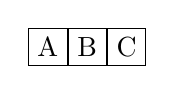
\begin{tikzpicture}
            \node [draw,rectangle](a)at(-1/2,0){A};
            \node [draw,rectangle](b)at(0,0){B};
            \node [draw,rectangle](c)at(1/2,0){C};     
        \end{tikzpicture}
        \caption{Initial state $s_{0}$}
        \label{fig:initial_state_in_BWD}
    \end{subfigure}
    \begin{subfigure}[t]{0.25\textwidth}
        \centering
        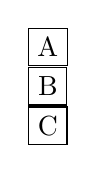
\begin{tikzpicture}
            \node [draw,rectangle](a)at(0,1){A};
            \node [draw,rectangle](b)at(0,1/2){B};
            \node [draw,rectangle](c)at(0,0){C};     
        \end{tikzpicture}
        \caption{Goal state $g$}
        \label{fig:goal_state_in_BWD}
    \end{subfigure}
    \caption{Initial state and Goal state for Blocks world domain}
    \label{fig:states_in_BWD}
\end{figure}

\noindent
In the beginning, we need to find a representation for the state and actions. For the state in blocks world is shown as below. For each state, the state should be \textbf{completely} specified based on the \textcolor{blue}{\textbf{Closed-World Assumption: any literal not mentioned in the description of the state are assumed to be false!}}.
\begin{outline}
    \1 On(b,x):
        \2 block b is on top of x, where x is another block 
    \1 Clear(x):
        \2 a block can be placed on the top of x
\end{outline}

\noindent
Thus, the initial state in Figure~\ref{fig:initial_state_in_BWD} are: $on(a,table)$, $on(b,table)$, $on(c,table)$, $clear(a)$, $clear(b)$, $clear(c)$. \textcolor{blue}{(Closed-World Assumption)} Additionally, the goal state in Figure~\ref{fig:goal_state_in_BWD} are: $clear(a)$, $on(a,b)$, $on(b,c)$, $on(c,table)$. \textcolor{blue}{(No Closed-World Assumption)}, we only need to satify the goal. (A state $s$ satisfies goal $g$ if it contains all literals in $g$, containing is okay, not exactly identified.)

\noindent
Next is the availble actions. It consists of \textbf{preconditions} and \textbf{effects}.
\begin{outline}
    \1 Preconditions: literals denoting what needs to be in the state for the action to be availble
    \1 Effects: literals denoting how the state is changing when action is applied
\end{outline}

\noindent
One of the avialble action is $move(b,x,y)$, meaning that move b from top of x to top of y. Anonther action can be $moveToTable(b,x)$ and $moveFromTable(b,x)$
\tabto{0mm} $move(b,x,y)$
\tabto{5mm} Preconditions:
\tabto{10mm} $on(b,x)$, $clear(b)$, $clear(y)$
\tabto{5mm} Effects:
\tabto{10mm} $\neg on(b,x)$, $\neg clear(y)$, $on(b,y)$, $clear(x)$ 
\tabto{0mm} $moveToTable(b,x)$
\tabto{5mm} Preconditions:
\tabto{10mm} $clear(b)$, $on(b,x)$
\tabto{5mm} Effects:
\tabto{10mm} $\neg on(b,x)$, $on(b,table)$, $clear(x)$
\tabto{0mm} $moveFromTable(b,x)$
\tabto{5mm} Preconditions:
\tabto{10mm} $clear(b)$, $clear(x)$
\tabto{5mm} Effects:
\tabto{10mm} $\neg on(b,table)$, $\neg clear(x)$, $on(b,x)$

\noindent
Why do we like formalism? Because it is easy for representation. STRIPS planning: finding a solution to the planning problem following a \textbf{state-based search:}
\begin{outline}
    \1 Init(\textcolor{orange}{where to start from})
    \1 Goal(\textcolor{orange}{when to stop searching})
    \1 Action(\textcolor{blue}{how to generate the "graph"})
\end{outline}

\noindent
When planning, there are two planning: 
\begin{outline}
    \1 Progression planning: forward state-based search \textcolor{red}{$\leftarrow$ mainly focus on}
    \1 Regression planning: backward state-based search
\end{outline}

\noindent 
The \textbf{\textcolor{blue}{pseudocode}} for progressing planning: - similar to backtracking
\begin{enumerate}
    \item Start from the initial state
    \item Check if the current state satisfies the goal
    \item Compute availble actions to the current state
    \item Compute the successor states
    \item Pick one of the \textbf{(not-visited)} successor states as the current state
    \item Repeat until a solution is found or the state space is exhausted \textcolor{red}{$\leftarrow$ similar to backtracking}
\end{enumerate}

\noindent
Is it guaranteed that progressive planning will find a solution if one exists? \textcolor{red}{$\leftarrow$ yes, if the state-space is finite} 

\noindent
But it will be very very slow, if we search the whole space-state (the worst case). \textcolor{red}{$\leftarrow$ heuristics needed!} We need heuristics that help progression planning pick the most promising states to investigate first

\subsection{Heuristics for STRIPS planning}
Analogy: $A^{*}$ search, evalution function = $f(s) = g(s) + h(s)$, where $g(s)$ from UCS and $h(s)$ from greedy search. Similar to the $A^{*}$ search, here we use $f(s)$ for STRIPS planning to pick the most promising one. Some of possible $h(s)$ and $g(s)$ can be as below. \emph{(Similarly, we need to check whether it is admissble heuristics to obtain the optimal solution)}
\begin{outline}
    \1 $g(s)$: number of literals that exists in the goal
    \1 $h(s)$: number of literals in the goal that are missing from s
\end{outline}

\noindent
The \textcolor{blue}{\textbf{pseudocode}} for \textcolor{blue}{\textbf{progressing planning}} applied with heuristics can be updated as below:
\begin{enumerate}
    \item Start from the initial state
    \item Check if the current state satisfies the goal
    \item Compute availble actions to the current state
    \item Compute the successor states
    \item Pick \textcolor{red}{\textbf{(the most promising}} successor states as the current state
    \item Repeat until a solution is found or the state space is exhausted \textcolor{red}{$\leftarrow$ similar to backtracking}
\end{enumerate}

\noindent
Alternatives: \textcolor{blue}{\textbf{pseudocode}} for \textcolor{blue}{\textbf{Regression planning }} is similar but invert the progressing planning:
\begin{enumerate}
    \item Start from the \textbf{goal} state as current state
    \item Check if the \textbf{initial state} satisfies the current state
    \item Compute the \textbf{relevant} and \textbf{consistent} actions for current state
    \item Compute the \textbf{predecessor} states (which is actually next state in this case)
    \item Pick \textcolor{red}{\textbf{(the most promising}} successor states as the current state
    \item Repeat until a solution is found from \textbf{goal state} to \textbf{initial state} or the state space is exhausted (no solution)
\end{enumerate}

\subsection{Summary}
\begin{enumerate}
    \item A generic formalism (easy to represent difficult space search, similar to ILP) for \textbf{representing} planning problem (a specific aspect in searching problem)
    \item Generic \textbf{search} procedures for finding a plan
    \begin{enumerate}
        \item Progressing planning (forward)
        \item Regression planning (backward, not discussed, only pseudocode)
    \end{enumerate}
    \item Application in many aspects, e.g., space, flight, robotics, etc.
\end{enumerate}


\pagebreak
\section{Markov Decision Process}
\subsection{Overview}
This section is about non-deterministic search, which is called stochastic search. First we can take Grid World as an example, which is shown below:

\begin{outline}
    \1 A maze-like problem
        \2 Agent move in the grid
        \2 Walls block the agent's path
    \1 Noisy movement - stochastic movement
        \2 $80\% \rightarrow$ correct direction, $20\% \rightarrow$ other (incorrect) directions.
    \1 The agent recives rewards each time step
        \2 Small living rewards (can be negative)
        \2 Big rewards at the end (negative or positive)
    \1 Goal: maximize sum of rewards
\end{outline}

\noindent
An MDP is defined as below. The MDP, the "markov" means actions outcomes depend only the current state, and the current, future and past are independent. It is similar to search, where the successor function could only depend on the current state (not the history). 
\begin{outline}
    \1 a set of states $s \in S$
    \1 a set of actions $ a \in A$
    \1 a transition function $T(s,a,s^{\prime})$
    \1 a reward function $R(s,a,s^{\prime})$
    \1 an initial state
    \1 some goal states (probably not)
\end{outline}

\noindent
Different between deterministic and stochastic search problem. In deterministic search, we want \textbf{an optimal path}, while in stochastic search, we want \textbf{an optimal policy $\pi: S \rightarrow A$,} where makes the agent becomes relfex agent. Each MDP state projects an expectimax-like search tree, similar to minimax but only with max layer and an addition chance state layer. 

\noindent
Some preference exists in MDP: \textbf{maximize} the sum of rewards $\rightarrow$ only max layer, prefer rewards \textbf{now} instead of later $\rightarrow$ discount factor $\gamma$ $\rightarrow$ indicating that values of rewards decay exponentially.

\noindent
Stopping criteria for MDP:
\begin{enumerate}
    \item Finite horizon (similar to depth-limited search), terminate episodes after a fixed T steps (e.g., life)
    \item Discounting: use $0 < \gamma < 1$: finally it will converge
    \item Absorbing state \textcolor{red}{$\leftarrow$ Question: do not understand!}
\end{enumerate}

\subsection{Solution for MDP}
\begin{outline}
    \1 Basic features
        \2 Set of states $S$
        \2 Initial state $s_{0}$
        \2 Set of actions $A$
        \2 Transition $P(s^{\prime}|s,a)$ (or $T(s,a,s^{\prime})$) \textcolor{red}{$\leftarrow$ probability}
        \2 Rewards $R(s,a,s^{\prime})$ (and discount $\gamma$)
    \1 MDP quantities so far
        \2 Policy = Choice of action for each state (Policy layer)
        \2 Utility = sum of (discount) rewards (Value layer)
\end{outline}

\begin{figure}[htbp]
    \centering
    \begin{tikzpicture}
        \node [draw,circle](s)at(3,5){};
        \node [draw,circle](sa)at(2,3){};
        \node [draw,circle](sas)at(3,1){};

        \draw[->] (s) -- (sa); 
        \draw[dashed,->] (s) -- (0,3);
        \draw[dashed,->] (s) -- (5,3);
        \draw[->] (sa) -- (sas);  
        \draw[dashed,->] (sa) -- (1,2);
        \draw[dashed,->] (sa) -- (4,2);
        \draw[->] (sas) -- (2,0);
        \draw[dashed,->] (sas) -- (0,0);
        \draw[dashed,->] (sas) -- (4,0);

        \draw (13/4,5) node[right]{$s$};
        \draw (5/2,4) node[right]{$a$};
        \draw (9/4,3) node[right]{$s,a$};
        \draw (5/2,2) node[left]{$s,a,s^{\prime}$};
        \draw (13/4,1) node[right]{$s^{\prime}$};
    \end{tikzpicture}
    \caption{Search tree of MDP}
    \label{fig:MDP_s_q_t_search_tree}
\end{figure}

\noindent
\begin{outline}
    \1 The value (utility) of $a$ state $s$:
        \2 $V^{\prime}(s)$ = expected utility starting in $s$ and acting optimally
    \1 The value (utility) of a q-state $(s,a)$:
        \2 $Q^{\prime}(s,a)$ = expected utility starting out having taken action $a$ from state $s$ and acting optimally (transition q-state).
    \1 The optimal policy:
        \2 $\pi^{\prime}(s)$ = optimal action from every state $s$
\end{outline}

\noindent
Recursive definition of value, \textbf{Bellman equations}:
\begin{outline}
    \1 $V^{*}(s) = \max\limits_a Q^{*}(s,a)$
    \1 $Q^{*}(s,a) = \sum_{s^{\prime}} T(s,a,s^{\prime}[R(s,a,s^{\prime}) + \gamma V^{*}(s^{\prime})])$
    \1 $V^{*}(s) = \max\limits_a \sum_{s^{\prime}} T(s,a,s^{\prime}) [R(s,a,s^{\prime}) + \gamma V^{*}(s^{\prime})]$
\end{outline}

\noindent 
The problem is still there, when to stop? Key idea: \textbf{time-limited values} by defining "life". Define $V_{k}(s)$ to be the optimal value of $s$ if the game ends in $k$ more time steps. Thus, there will be \textbf{value iteration} and \textbf{policy iteration}.

\subsection{Value iteration}
The complexity of each value iteration is $O(S^{2} \times A)$
\begin{enumerate}
    \item Start with $V_{0}(s) = 0$: no time steps left means an expected reward sum of zero.
    \item Given vector of $V_{k}(s)$ values, do one ply of expectimax from each state: $V_{k+1}(s) \leftarrow \max\limits_a \sum_{s^{\prime}} T(s,a,s^{\prime}) [R(s,a,s^{\prime}) + \gamma V_{k}(s^{\prime})]$
    \item Repeat until convergence
\end{enumerate}

\noindent
Some problems with value iteration:
\begin{enumerate}
    \item It is slow - with complexity $O(S^{2} \times A)$ per iteration
    \item The "max" at each state rarely changes
    \item The policy (a set of actions) often \textbf{converges long} before the values
\end{enumerate}

\subsection{Policy iteration}
\subsubsection{Fixed policy}
If we try a fixed policy $\pi(s)$, then the tree will be simpler - only one action per state, compared to that the expectimax tree max over all actions to compute the optimal values. Define the utility (V function) of a state $s$, under a fixed policy $\pi$, the value function will be: $V^{\pi}(s) = \sum_{s^{\prime}} T(s,\pi(s),s^{\prime}) [R(s,\pi(s),s^{\prime}) + \gamma V^{\pi}(s^{\prime})]$.

\noindent
How do we calcualte the V's for a fixed policy $pi$? 
\begin{outline}
    \1 $V_{0}^{\pi} (s) = 0$
    \1 $V_{k+1}^{\pi} (s) \leftarrow \sum_{s^{\prime}} T(s,\pi(s),s^{\prime}) [R(s,\pi(s),s^{\prime}) + \gamma V_{k}^{\pi} (s^{\prime})]$, with $O(S^{2})$
\end{outline}

\subsubsection{Policy extraction}
After obtaining values or q-values from the current map, we can extract the policy from a value-map or q-value-map, thus we have two basic algorithm for extracting policy (a set of actions): computing actions from values or computing actions from Q-values. It is obvious that \textbf{actions are easier to select from q-values than values}, because $V(s) = arg\max\limits_a Q(a,s)$.
\begin{outline}
    \1 Computing actions from values:
        \2 $\pi^{*}(s) = arg\max\limits_a \sum_{s^{\prime}} T(s,a,s^{\prime}) [R(s,a,s^{\prime}) + \gamma V^{*}(s^{\prime})]$
    \1 Computing actions from Q-values:
        \2 $\pi^{*}(s) = arg\max\limits_a Q^{*}(s,a)$
\end{outline}

\subsubsection{Policy iteration}
Alternative approach for optimal values: (policy fixed instead of expectimax search). Optimal and can converge faster under some conditions compared to expectimax search.
\begin{enumerate}
    \item Step 1: Policy evaluation: calculate utilities for some \textbf{fixed policy} (not optimal utilities!) until \textbf{convergence}
    \item Step 2: Policy improvment: update policy using one-step look-ahead with resulting converged (not optimal but will be finally) utilities as \textbf{future values}
    \item Repeat steps until policy converges
\end{enumerate}

\noindent
For more details in policy iteration: evaluation is for finding values by fixed policy $\pi_{i}: V^{\pi_{i}}(s) \rightarrow V^{\pi_{i}}(s^{\prime})$, and improvment is for extracting policy by fixed values $V^{\pi_{i}}(s): \pi_{i} \rightarrow \pi_{i+1}$. And repeat these two processes until convergence of policy (policy (all actions) is not changed anymore.)
\begin{outline}
    \1 \textbf{Evaluation}: for fixed current policy $\pi$, find values with policy evaluation:
        \2  $V_{k+1}^{\pi_{i}}(s) \rightarrow \sum_{s^{\prime}} T(s,\pi_{i}(s),s^{\prime}) [R(s,\pi_{i}(s),s^{\prime}) + \gamma V_{k}^{\pi_{i}}(s^{\prime})]$
    \1 \textbf{Improvement}: for fixed values, get a better policy using policy extraction
        \2 $\pi_{i+1}(s) = arg\max\limits_a \sum_{s^{\prime}} T(s,a,s^{\prime}) [R(s,a,s^{\prime}) + \gamma V^{\pi_{i}}(s^{\prime})]$
\end{outline}

\subsection{Value vs. Policy iteration}
Both value iteration and policy iteration compute the same thing (all optimal values), but with different efficiency under various situation. Both are dynamic programs for solving MDPs.
\begin{enumerate}
    \item In value iteration
    \begin{enumerate}
        \item Every iteration updates both the values and \textbf{(implicitly)} the policy \textcolor{red}{$\leftarrow$ only value function explicitly}
        \item We do not track the policy, but taking the max over actions implicity recomputes it, just not show a policy map, only show a value map. 
    \end{enumerate}
    \item In policy iteration
    \begin{enumerate}
        \item In each turn, we intersectly \textcolor{blue}{\textbf{update the utility with fixed policy}}, and \textcolor{blue}{\textbf{extract the policy with fixed updated utility}} (each turn is fast since we only consider one action not all of them instead of expectimax search/ value interation) \textcolor{red}{$\leftarrow$ both value and policy function explicitly}
        \item After the policy is evaluated, the new policy is chosen
        \item Using new policy to continue till the stopping criteria (life-limit or threshold)
        \item Here we not only check the V-value/Q-value but also check the policy, show both V-value/Q-value map and policy map.
    \end{enumerate}
\end{enumerate}

\subsection{Summary}
\begin{enumerate}
    \item Different methods are introduced
    \begin{enumerate}
        \item Compute optimal values (whole): \textbf{value iteration} or \textbf{policy iteration}
        \item Compute values from a particular policy: use \textbf{policy evaluation}
        \item Extract policy from a set of values: use \textbf{policy extraction} \textcolor{red}{(one-step lookahead?)}
    \end{enumerate}
    \item However, both value iteration and policy iteration are similar
    \begin{enumerate}
        \item They are basically are variations of \textbf{Bellman updates}
        \item They \textbf{all} use \textbf{one-step lookahead expectimax fragments} (no matter value iteration, but also policy iteration)
        \item Difference in \textbf{max over actions (value iteration)} or \textbf{fixed policy (policy iteration)}, just different efficiency under different situation, sometime value iteration better, sometime policy iteration better, \textcolor{purple}{it depends on your own domain knowledge!}
    \end{enumerate}
\end{enumerate}

\pagebreak
\clearpage


\end{document}
